\documentclass[12pt]{article}

\usepackage[a4paper,  top=1.3in, bottom=1.4in, left=1.4in, right=1.5in]{geometry}

\usepackage[utf8]{inputenc}
\usepackage[T1]{fontenc}
\usepackage{amsmath}
\usepackage{amsfonts}
\usepackage{amssymb}
\usepackage{tabularx}
\usepackage{array}
\usepackage{float}

\usepackage{graphicx, float}
\usepackage{adjustbox}
\graphicspath{{images/}}

\renewcommand{\figurename}{Slika}
\renewcommand{\tablename}{Tabela}


\renewcommand{\baselinestretch}{1.2} % Line spacing

% Parskip and parindent
\setlength{\parindent}{0pt} % Begin of paragraph indentation
\setlength{\parskip}{1em} % Paragraph spacing

%--- for references ---------
\usepackage[
    backend=biber,
    style=numeric,
    sorting=none
    ]{biblatex}

\addbibresource{bibliography.bib}
\AtBeginBibliography{\vspace*{10pt}}
%----------------------------

%----------- toc ------------------------
\usepackage{tocloft}
\usepackage{fancyhdr}
% \setlength{\cftbeforesecskip}{0pt} % Adjust the spacing before section entries
% \setlength{\cftbeforesubsecskip}{0pt} % Adjust the spacing before subsection entries
%----------------------------------------

\begin{document}
\pagenumbering{gobble}  % Suppress page numbers initially

% Title Page
\newgeometry{top=1in, bottom=1in, left=1in, right=1in} % New margins for title page
\begin{titlepage}
    \begin{center}
        
        % add your university logo here
        % negative value moves the logo up
        \vspace*{-1in}
        
\includegraphics[width=0.4\textwidth]{raf_logo.png}

        % set font size to 14pt
        \vspace{1in}
        \Large
        \textbf{Tema}
        
        % set horizontal margin for the title to 1.5in and center it
        \vspace{1in}
        \Huge
        \textbf{Skaliranje sistema za rezervaciju: Analiza različitih arhitekturalnih pristupa i strategija za skaliranje servisa}
        
        \vspace{1in}


            \fontsize{17pt}{17pt}\selectfont
            \textbf{Kurs: Praktikum in računarstva u oblaku} \\
            \vspace*{1.5in}
            
            \begin{center}
            \normalsize
            \begin{tabular}{p{0.75\textwidth} p{0.5\textwidth}}
                \fontsize{14pt}{18pt}\selectfont   
                \textbf{Mentor:} & 
            
                \fontsize{14pt}{18pt}\selectfont
                \textbf{Student:} \\
                prof. Mirjana Radivojević & Vanja Kovinić \\
            \end{tabular}
            \end{center}

            \vspace*{\fill}

            \normalsize
            Beograd, 2025.


            
        \end{center}
    \end{titlepage}
    \restoregeometry % Restore original margins

    \newpage
    \newgeometry{top=1.3in, bottom=2.2in, left=1.4in, right=1.4in} % New margins for title page
    \renewcommand{\contentsname}{Sadržaj}
    \tableofcontents{}

    \newpage
    \clearpage             % Move to a new page
    \pagenumbering{arabic} % Start using Arabic numerals
    \setcounter{page}{1}   % Set the counter to 1

    \newpage
    \section{Uvod}
    \subsection{Problem i motivacija}

    Upravljanje resursima u modernim poslovnim okruženjima predstavlja ključni izazov za 
    efikasno funkcionisanje organizacija. Rezervacija sala za sastanke, kao jedan od najčešćih 
    operativnih procesa, često je opterećena manuelnim postupcima koji dovode do konflikata 
    u rasporedu, duplih rezervacija i neoptimalnog korišćenja prostora.

    U konkretnom slučaju koji je analiziran u ovom radu, vlasnik poslovnog centra koji 
    iznajmljuje sale za sastanke suočavao se sa potpunim odsustvom digitalnog sistema 
    za rezervacije. Ceo proces rezervacije bio je centralizovan kroz jednu sekretaricu koja 
    je putem email komunikacije primala zahteve, proveravala dostupnost i potvrđivala 
    rezervacije. Ovakav pristup stvorio je više kritičnih problema:

    \begin{itemize}
        \item \textbf{Nedovoljna preglednost}: Klijenti nisu imali mogućnost da vide raspoloživost sala u realnom vremenu, što je otežavalo planiranje.
        \item \textbf{Ograničena fleksibilnost}: Promene u rasporedu bile su teške za implementaciju, što je dovodilo do dodatnih konflikata.
        \item \textbf{Neproduktivno trošenje vremena}: Značajan deo radnog vremena sekretarice bio je posvećen repetitivnim zadacima umesto obavljanju kompleksnih i strateških zadataka.
        \item \textbf{Neprofesionalan imidž}: Manuelni proces ostavljao je utisak zastarele i neorganizovane kompanije kod klijenata.
        \item \textbf{Nedostatak analitike}: Bez digitalnog sistema, bilo je nemoguće pratiti trendove korišćenja sala, što je otežavalo donošenje poslovnih odluka.
        \item \textbf{Skalabilnost problema}: Sa rastom broja klijenata, sistem je postajao sve manje održiv.
    \end{itemize}

    \subsection{Tehnologije i pristup}

    Implementacija sistema zasniva se na \textbf{Java} \cite{java_language} programskom jeziku 
    i \textbf{Spring Boot} \cite{spring_boot} 
    okruženju, koje čini osnovni sloj aplikacione logike. Uz savremene pristupe 
    kontejnerizacije i principe razvoja \textit{cloud-native} aplikacija, postignuta je 
    visoka prenosivost i konzistentnost sistema u različitim okruženjima. \textbf{Docker} \cite{docker} je 
    korišćen za pakovanje i izolaciju aplikacije, dok je \textbf{GitHub Actions} \cite{github} iskorišćen 
    za potpunu automatizaciju procesa kontinuirane integracije i isporuke (\textbf{\textit{CI/CD}} \footnote{\textit{CI/CD - Continuous Integration/Continuous Deployment}}).

    Aplikacija je postavljena na \textbf{Netcup cloud} \cite{netcup} infrastrukturu, čime je obezbeđeno ekonomično i 
    skalabilno rešenje za produkcijski hosting.

    Ključne tehnologije korišćene u projektu su:
    \begin{itemize}
    \item \textbf{Razvojna platforma:} \textbf{Java} i \textbf{Spring Boot}, sa implementacijom \textit{RESTful API}-ja\footnote{\textit{RESTful API (Representational State Transfer)} je pristup pravljenja web servisa koji koriste \textit{HTTP} protokol za komunikaciju i manipulisanje resursima na serveru.}
 za komunikaciju između klijenta i servera
    \item \textbf{Kontejnerizacija:} \textbf{Docker}, za pakovanje aplikacije i izolaciju od okruženja  
    \item \textbf{Orkestracija:} \textbf{Docker Compose}, za upravljanje više kontejnera u okviru jednog sistema  
    \item \textbf{Automatizacija (CI/CD):} \textbf{GitHub Actions}, za automatsko testiranje i postavljanje aplikacije na server  
    \item \textbf{Baza podataka:} Relaciona baza podataka (\textbf{MySQL} \cite{mysql}) pokrenuta u posebnom kontejneru  
    \item \textbf{Cloud infrastruktura:} \textbf{Netcup VPS}, korišćen za postavljanje i pokretanje sistema u produkciji
    \end{itemize}
    
    \newpage
    Poseban akcenat stavljen je na automatizaciju procesa postavljanja aplikacije, 
    što omogućava brzo isporučivanje novih funkcionalnosti kroz jednostavno slanje izmena u 
    repozitorijum (\textit{git push}). Ovakav pristup značajno smanjuje vreme potrebno za 
    implementaciju i testiranje izmena.
    Izvorni kod i konfiguracija dostupni su na \textbf{GitHub} platformi \footnote{\url{https://github.com/Kovelja009/conf_room}}.

    \section{Arhitekturni obrasci: Monolit vs Mikroservisi}
    \subsection{Teoretske osnove}

    \textbf{Monolitna arhitektura} predstavlja tradicionalni pristup razvoju softverskih sistema
    , pri kojem se celokupna funkcionalnost implementira u okviru jedne celovite i 
    zajednički postavljene aplikacije. U ovom modelu, sve komponente sistema - upravljanje 
    korisnicima, poslovna logika, pristup bazi podataka i prikaz podataka 
    (interfejs) - integrisane su unutar jednog izvršnog procesa. Komunikacija između delova 
    sistema odvija se putem direktnih poziva funkcija unutar iste aplikacije, što može 
    doprineti boljim performansama, ali istovremeno dovodi do 
    jake povezanosti (\textit{tight coupling}) između modula i smanjenja fleksibilnosti u 
    razvoju i održavanju.

    S druge strane, \textbf{mikroservisna arhitektura} predstavlja savremeniji pristup 
    koji uvodi koncept distribuiranih sistema. Aplikacija se u ovom modelu sastoji od niza 
    nezavisnih servisa, od kojih je svaki odgovoran za tačno određenu poslovnu funkcionalnost. 
    Svaki mikroservis poseduje sopstvenu bazu podataka i može se razvijati, testirati i 
    postavljati potpuno nezavisno od ostalih servisa. Ovakav pristup omogućava veću fleksibilnost 
    i skalabilnost, ali istovremeno uvodi dodatnu složenost, naročito u oblastima kao što su 
    otkrivanje servisa (\textit{service discovery}), međuservisna komunikacija i upravljanje 
    transakcijama koje obuhvataju više servisa.

    \newpage
    U kontekstu razvoja za \textit{cloud} okruženje, oba arhitekturna pristupa mogu se 
    uspešno implementirati uz korišćenje kontejnerskih tehnologija. 
    \textbf{Docker} omogućava konzistentno postavljanje aplikacija bez obzira na konkretno 
    okruženje u kojem se izvršavaju, dok platforme za orkestraciju poput 
    \textbf{Kubernetesa} \cite{kubernetes} nude napredne mogućnosti za upravljanje servisima, automatsko 
    skaliranje i raspodelu opterećenja. Konačan izbor arhitekture zavisi od specifičnih zahteva 
    aplikacije, veličine i organizacije razvojnog tima, kao i infrastrukturnih i operativnih 
    ograničenja.
    
    \newpage
    \subsection{Komparativna analiza}

    Poređenje monolitne i mikroservisne arhitekture prikazano je u Tabeli \ref{tabela:monolit_vs_mikroservisi}. 
    Ova tabela sumira ključne aspekte oba pristupa, uključujući skalabilnost, 
    izolaciju grešaka, kompleksnost razvoja, performanse, složenost \textit{CI/CD} procesa i 
    tehnologije koje se koriste. 

    \hspace{0.4cm}
    \begin{table}[H]    
    \centering
    \small
    \renewcommand{\arraystretch}{1.4}
    \begin{tabularx}{\textwidth}{
        |>{\raggedright\arraybackslash}>{\hsize=0.8\hsize}X
        |>{\raggedright\arraybackslash}>{\hsize=0.8\hsize}X
        |>{\raggedright\arraybackslash}>{\hsize=0.8\hsize}X
        |>{\raggedright\arraybackslash}>{\hsize=1.6\hsize}X|}
            \hline
            \textbf{Aspekt} & \textbf{Monolit} & \textbf{Mikroservisi} & \textbf{Kontekst primene} \\
            \hline
            Skalabilnost & Vertikalna & Horizontalna & Monolit za mali broj korisnika, mikroservisi za veći broj i opterećenje \\
            \hline
            Izolacija grešaka & Niska & Visoka & Manji sistemi mogu tolerisati jednu tačku otkaza \\
            \hline
            Kompleksnost razvoja & Niska & Visoka & Monolit za male timove, mikroservisi za kompleksne sisteme \\
            \hline
            Performanse & Brže (lokalni pozivi) & Sporije (mreža) & Direktan metod vs \textit{HTTP/REST} \\
            \hline
            \textit{Deployment} & Jednostavan & Složen & \textit{CI/CD} zahteva više skripti za mikroservise \\
            \hline
            Komunikacija & Lokalni pozivi & Međuservisna komunikacija & Direktan pristup vs API pozivi \\
            \hline
            \textit{CI/CD} složenost & Jedan tok & Više tokova & Veći broj servisa, nezavisna postavljanja \\
            \hline
            Tehnologije & Jedinstven stek & Potencijalno više tehnologija & Manji timovi preferiraju doslednost \\
            \hline
            Monitoring & Centralizovan & Distribuiran & Lakše praćenje u monolitu \\
            \hline
            \end{tabularx}
            \caption{Uporedna analiza monolitne i mikroservisne arhitekture}
        \label{tabela:monolit_vs_mikroservisi}


    \end{table}
    \newpage

    \subsection{Faktori za donošenje odluke}

    Izbor arhitekture samog servisa zavisi od više povezanih faktora koje je potrebno pažljivo 
    analizirati u konkretnom poslovnom i tehničkom kontekstu:

    \subsubsection*{Struktura tima i organizacioni faktori}

    \textit{Conway-ev zakon} sugeriše da arhitektura sistema odražava strukturu komunikacije 
    unutar organizacije koja ga razvija. U slučaju malih timova (npr. dva programera), 
    što je karakteristično za analizirani projekat, \textbf{monolitna arhitektura} se često 
    pokazuje kao optimalan izbor jer omogućava:
    \begin{itemize}
        \item jedinstveno razvojno okruženje bez dodatnog koordinacionog opterećenja između \textit{frontend} i \textit{backend} programera,
        \item pojednostavljeno orkestriranje koda - direktan pristup zajedničkom kodu,
        \item brže donošenje odluka bez zavisnosti između timova i dileme oko vlasništva nad servisima.
    \end{itemize}

    \subsubsection*{Količina saobraćaja i zahtevi u pogledu performansi}

    Očekivano opterećenje predstavlja ključni faktor u izboru arhitekture:
    \begin{itemize}
        \item \textbf{Nizak nivo saobraćaja} (desetine istovremenih korisnika): performanse monolita su 
        u potpunosti dovoljne, dok bi mrežna latencija karakteristična za mikroservise predstavljala 
        nepotreban trošak.
        \item \textbf{Srednji nivo saobraćaja} (stotine korisnika): prelazna zona u kojoj su oba 
        pristupa moguća i zavise od dodatnih faktora.
        \item \textbf{Visok nivo saobraćaja} (hiljade i više korisnika): mikroservisna arhitektura 
        omogućava horizontalno skaliranje i bolje upravljanje opterećenjem, što je ključno za 
        očuvanje performansi i dostupnosti sistema.
    \end{itemize}

    \subsubsection*{Brzina razvoja i učestalost \textit{deployment}-a aplikacije}

    Učestalost \textit{deployment}-a značajno utiče na odabir arhitekture:
    \begin{itemize}
        \item \textbf{Čest \textit{deployment}} (npr. više puta dnevno tokom razvoja): automatizacija 
        \textit{CI/CD} procesa postaje od suštinskog značaja, ali je jednostavnija za 
        implementaciju u okviru monolita.
        \item \textbf{Koordinacija više servisa}: mikroservisi zahtevaju naprednu orkestraciju kako 
        bi se obezbedila sinhronizovana postavljanja.
    \end{itemize}

    \subsubsection*{Tehnološka ograničenja i operativna zrelost}

    DevOps kapaciteti organizacije predstavljaju značajan ograničavajući faktor:
    \begin{itemize}
        \item \textbf{Ograničeno operativno iskustvo}: postavljanje i nadgledanje monolita je 
        jednostavnije i zahteva manje alata i znanja.
        \item \textbf{Napredni operativni kapaciteti}: mikroservisi zahtevaju složenije mehanizme 
        za otkrivanje servisa (\textit{service discovery}), balansiranje 
        opterećenja (\textit{load balancing}) i distribuirani nadzor sistema.
        \item \textbf{Kompleksnost komunikacije između servisa}: direktni pozivi metoda naspram 
        \textit{HTTP/REST API} poziva za razmenu podataka.
    \end{itemize}

    Konačna odluka treba da uspostavi ravnotežu između trenutnih potreba za brzinom razvoja i 
    dugoročnih zahteva za skalabilnošću, uzimajući u obzir sposobnosti postojećeg tima i 
    predviđeni rast sistema.

    \newpage
    \section{Funkcionalnosti sistema}

    Razvijeni sistem za rezervaciju konferencijskih sala obuhvata tri ključne funkcionalne celine implementirane kao deo jedinstvene \textit{Spring Boot} aplikacije, čime je obezbeđen kompletan tok obrade zahteva korisnika, od autentifikacije do obaveštavanja putem elektronske pošte.

    \subsection{Servis za autentifikaciju korisnika}

    Mehanizam autentifikacije zasniva se na JWT \footnote{\textit{JSON Web Token}} standardu, koji 
    omogućava sesije bez čuvanja stanja (\textit{stateless}), što je pogodno za skalabilna 
    \textit{cloud} rešenja. U sistemu su definisane dve korisničke uloge:
    \begin{itemize}
    \item \textbf{Korisnik (USER)} - mogućnost kreiranja i upravljanja sopstvenim rezervacijama
    \item \textbf{Menadžer (MANAGER)} - administrativna ovlašćenja: kreiranje korisničkih naloga i pregled analitičkih izveštaja
    \end{itemize}

    Registraciju korisnika vrši isključivo menadžer, čime se sprečava nekontrolisan pristup sistemu. Nakon registracije, korisniku se automatski prosleđuje elektronska poruka sa pristupnim podacima. Mehanizam za promenu lozinke funkcioniše putem bezbedne email procedure, gde se zahtevi za reset lozinke proveravaju na osnovu korisničkog imena i registrovane adrese elektronske pošte.

    \newpage
    \subsection{Servis za upravljanje rezervacijama}

    Interfejs baziran na kalendarskom prikazu omogućava korisnicima intuitivan odabir termina. Sistem 
    koristi naprednu logiku za detekciju konflikata, koja pored vremenskog preklapanja uvažava i 
    obavezne periode za pripremu i čišćenje između rezervacija. U slučaju konflikta, korisniku se 
    nudi objašnjenje kako bi u skladu sa tim prilagodio svoje planove.

    Dodatno, korisnicima je omogućeno izmenjivanje i otkazivanje rezervacija koje još nisu započete, čime se obezbeđuje fleksibilnost u planiranju.

    \subsection{Servis za elektronsku poštu}

    Sistem automatski generiše obaveštenja putem elektronske pošte za sledeće slučajeve:
    \begin{itemize}
    \item Potvrda kreiranja, izmene i otkazivanja rezervacija
    \item Dobrodošlica korisniku sa pristupnim podacima
    \item Obaveštavanja o ažuriranjima naloga korisnika
    \item Izveštaji i obaveštenja za administrativne korisnike
    \end{itemize}

    Poruke se generišu na osnovu unapred definisanih šablona koji uključuju dinamičke 
    informacije (datum, vreme, naziv korisnika), kao i vizuelne elemente u skladu sa brendom firme.

    \newpage
    \subsection{Baza podataka}

    Struktura baze zasniva se na relacionom modelu, a koristi se \textit{MySQL} kao sistem za upravljanje 
    bazom podataka. Ključne tabele se mogu videti na \\ Slici \ref{fig:baza_struktura}.

    \begin{figure}[h!]
        \vspace{0.5cm}
        \centering
        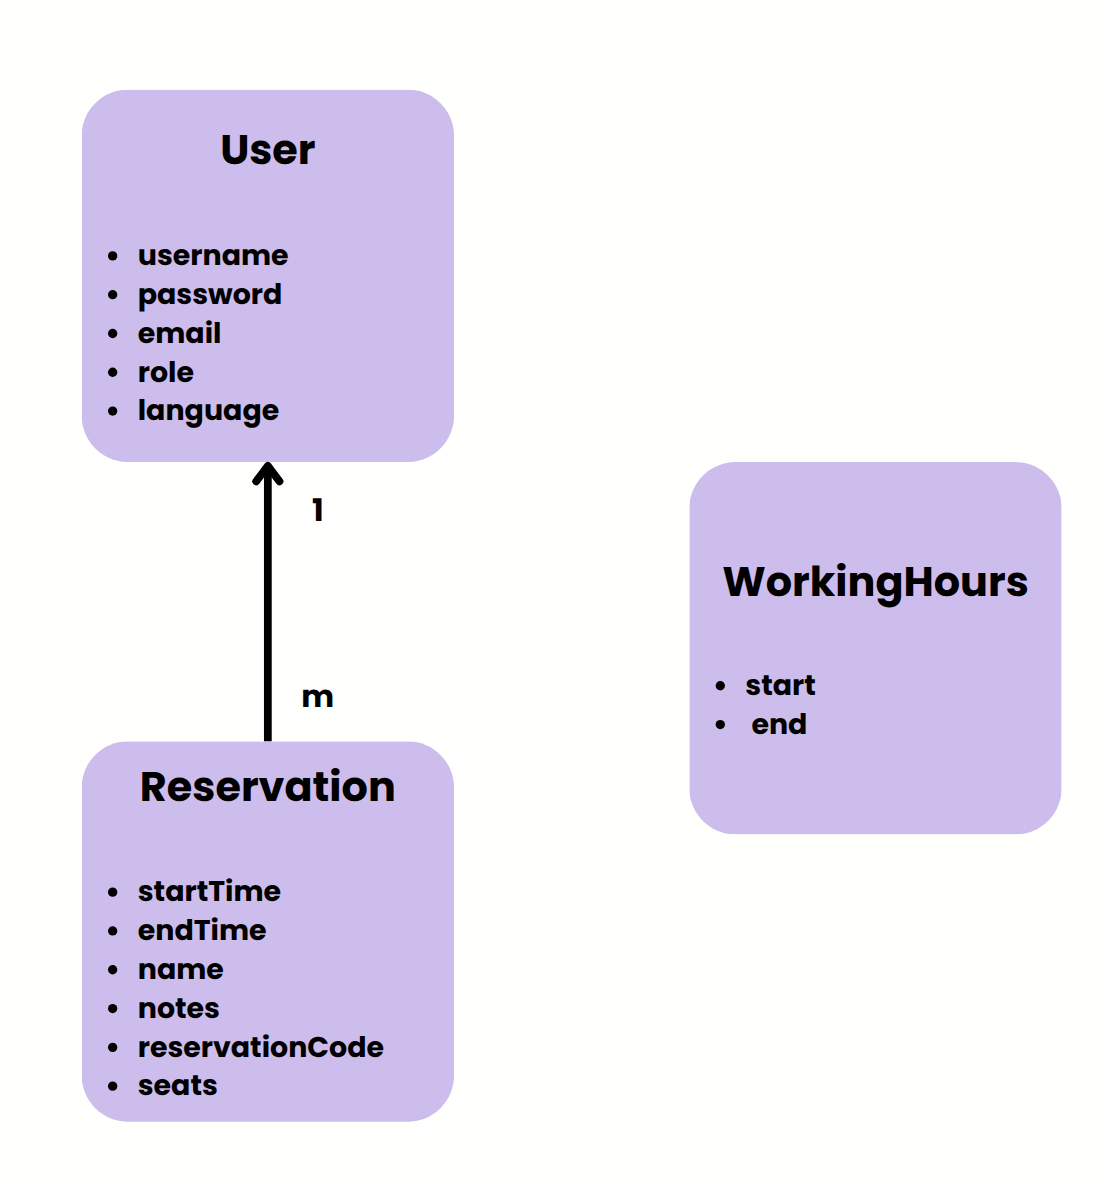
\includegraphics[width=0.7\textwidth]{db.png}
        \caption{Struktura baze podataka}
        \label{fig:baza_struktura}
    \end{figure}

    Tabela \texttt{Working\_Hours} omogućava definisanje različitih radnih termina u 
    zavisnosti od sezonskih rasporeda, praznika i posebnih događaja. Sistem je projektovan sa 
    mogućnošću proširenja za podršku više sala, uz minimalan uticaj na postojeću logiku.

    \newpage

    \subsection{Arhitektura sistema}

    Pregled arhitekture sistema prikazan je na Slici \ref{fig:arhitektura_sistema}.

    \begin{figure}[h!]
        \vspace{0.5cm}
        \centering
        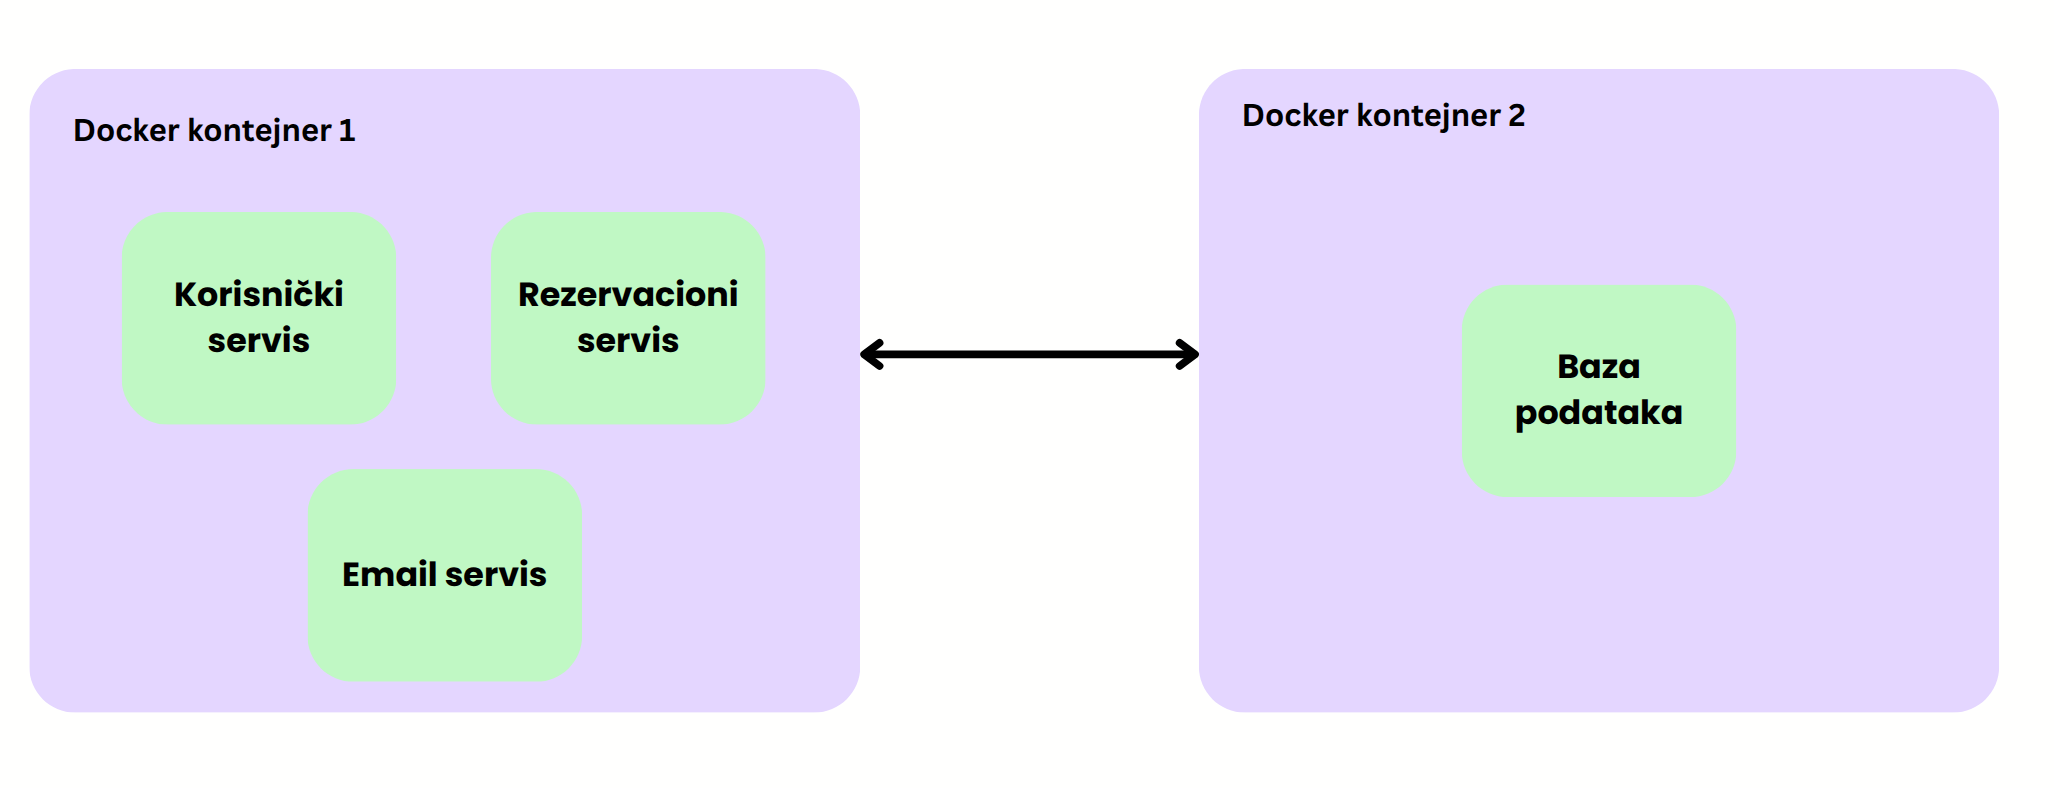
\includegraphics[width=1.0\textwidth]{sistem.png}
        \caption{Dva \textit{Docker} kontejnera su povezana preko virtualne mreže}
        \label{fig:arhitektura_sistema}
    \end{figure}

    \subsubsection*{Aplikacioni kontejner (monolitna arhitektura)}

    Svi servisi (autentifikacija, rezervacije, elektronska pošta) implementirani su kao deo jedne \textit{Spring Boot} aplikacije i distribuiraju se kao jedinstveni \texttt{JAR} \footnote{Java ARchive} fajl. Prednosti ovog pristupa uključuju:

    \begin{itemize}
    \item Direktni pozivi metoda unutar procesa (bez mrežne latencije)
    \item Zajednički kontekst transakcija i konzistentnost podataka
    \item Jedinstveni mehanizam za logovanje i rukovanje greškama
    \item Centralizovano upravljanje konfiguracijom
    \end{itemize}

    \newpage

    Docker fajl za izgradnju kontejnera izgleda ovako:

    \begin{verbatim}
    FROM openjdk:17-jdk-slim
    COPY conf_room-0.0.1-SNAPSHOT.jar app.jar
    EXPOSE 8082
    ENTRYPOINT ["java", "-jar", "app.jar"]
    \end{verbatim}

    \subsubsection*{Kontejner sa bazom podataka}

    Baza podataka koristi \textit{MySQL 8.0}, postavljena u posebnom kontejneru sa sledećim karakteristikama:
    \begin{itemize}
    \item Provera ispravnosti startovanja sistema (\textit{health check})
    \item Upotreba trajnih volumena za očuvanje podataka
    \end{itemize}
    
    \subsubsection*{Mreža i komunikacija između kontejnera}

    Komunikacija između kontejnera odvija se unutar prilagožene \textbf{Docker} mreže, što omogućava:
    \begin{itemize}
      \item Otkrivanje servisa po imenu kontejnera
      \item Izolaciju mrežnog sloja od host sistema
      \item Konfigurisanje putem \texttt{.env} fajla
      \item Bezbednu razmenu podataka unutar sistema
    \end{itemize}

    \subsection{Automatizacija putem CI/CD procesa}

    \subsubsection*{GitHub Actions automatizacija}

    Proces automatskog postavljanja aplikacije pokreće se svakim slanjem izmena na glavnu granu repozitorijuma (\texttt{main}). Sledeći koraci se izvršavaju automatski:
    \begin{itemize}
    \item Preuzimanje koda i izgradnja aplikacije (\textit{Maven build})
    \item Usmeravanje konekcije ka serveru (\textit{SSH setup})
    \item Čišćenje prethodnih fajlova i prebacivanje novih
    \item Ponovno pokretanje kontejnera sa novom verzijom
    \end{itemize}

    Bezbednost je obezbeđena korišćenjem enkriptovanih ključeva i promenljivih okruženja (\textit{GitHub Secrets}).

    \subsubsection*{Prednosti automatizovanog postavljanja}

    Vreme potrebno za postavljanje aplikacije smanjeno je sa oko 15 minuta na manje od 3 minuta, 
    što značajno ubrzava testiranje novih funkcionalnosti. Automatizacija takođe eliminiše problem 
    razlika između lokalnog i produkcionog okruženja.

    \newpage

    \subsection{Postavljanje aplikacije na cloud (Netcup)}

    Sistem je postavljen na \textbf{Netcup VPS} okruženje, koje predstavlja povoljno rešenje za 
    očekivani broj korisnika. Izvršavanje aplikacije direktno 
    preko \textit{Spring Boot runtime} okruženja omogućava efikasno korišćenje resursa.

    Trenutni nivo \textit{VPS}-a je dovoljan za postojeći obim saobraćaja, 
    a sistem je projektovan tako da podržava buduće unapređenje u skladu sa rastom broja korisnika.

    \section{Razlozi za izbor monolitne arhitekture}

    \subsection{Analiza konteksta}

    Izbor arhitekture u ovom projektu rezultat je specifičnih poslovnih i tehničkih ograničenja, na osnovu kojih je monolitna arhitektura predstavljala najracionalnije rešenje u datim okolnostima.

    \subsubsection*{Zahtevi klijenta i očekivano opterećenje sistema}

    Klijent (poslovni centar) postavio je jasne funkcionalne zahteve:
    \begin{itemize}
    \item Očekivani broj istovremenih korisnika: desetine korisnika, što je znatno ispod praga koji bi opravdao potrebu za mikroservisnom arhitekturom
    \item Scenario sa jednom zgradom i jednom salom - jednostavne \textit{CRUD} \footnote{Create, Read, Update, Delete} operacije
    \item Predvidivost nivoa opterećenja servisa (tokom radnog vremena)
    \item Potreba za brzim i ekonomičnim rešenjem
    \end{itemize}

    Iz \textit{ROI} \footnote{Return on Investment} aspekta, uvođenje složenije distribuirane arhitekture bi predstavljalo 
    bespotrebno komplikovanje u odnosu na realne potrebe.

    \subsubsection*{Ograničenja u vezi sa timom i rokovima}

    Sistem je razvijen u okviru dvočlanog tima (frontend i backend/DevOps), što je u velikoj meri uticalo na izbor arhitekture:
    \begin{itemize}
    \item Troškovi koordinacije u mikroservisnim okruženjima bi bili nesrazmerno visoki za ovako mali tim
    \item Jedinstvena baza koda olakšava razmenu znanja i sinhronizaciju razvoja
    \item Vremenski okvir od samo mesec i po dana predstavljao je dodatno ograničenje koje isključuje primenu kompleksnih arhitektura
    \end{itemize}

    U skladu sa Konvejovim zakonom (\textit{Conway's Law} \cite{ConwaysLaw}) - arhitektura softvera je povezana sa strukturom tima i organizacije.
    U našem slučaju, jedan član je odgovoran za frontend, a drugi za backend i DevOps aspekte, što je dodatno favorizovalo monolitnu arhitekturu.

    \newpage

    \subsection{Prednosti monolitne arhitekture u datom kontekstu}

    \subsubsection*{Prednosti u razvoju i implementaciji}

    Monolitni pristup omogućio je jedinstveno razvojno okruženje:
    \begin{itemize}
    \item Komunikacija unutar procesa: direktni pozivi metoda umesto \texttt{HTTP} poziva (kašnjenje reda veličine mikrosekundi u poređenju sa milisekundama)
    \item Zajednički kontekst transakcija: \textit{ACID} \footnote{\textit{Atomicity, Consistency, Isolation, Durability}} svojstva obuhvataju sve komponente
    \item Automatska konfiguracija putem \textit{Spring Boot}-a
    \end{itemize}

    \subsubsection*{Operativna jednostavnost}

    Postavljanje i održavanje aplikacije znatno su jednostavniji:
    \begin{itemize}
    \item Jedinstveni artefakt za izgradnju, testiranje i postavljanje
    \item Nadzor i logovanje vrše se u okviru jedne aplikacione instance
    \item Niski infrastrukturni troškovi - dovoljan osnovni VPS bez potrebe za platformama za orkestraciju
    \end{itemize}

    \newpage
    
    \subsection{Kritički osvrt}

    \subsubsection*{Analiza kompromisa}

    Ograničenja monolitne arhitekture su poznata i svesno prihvaćena:
    \begin{itemize}
    \item Skalabilnost: vertikalna skalabilnost zadovoljava trenutne potrebe; horizontalna skalabilnost se može uvesti kasnije
    \item Tehnološka ograničenja: svi servisi koriste isti stek tehnologija
    \item Skaliranje tima: ovakav pristup nije pogodan za veliki tim, ali je optimalan za dvočlani tim
    \item Održavanje: monolit može postati teško održiv sa rastom broja funkcionalnosti
    \end{itemize}

    \subsubsection*{Kada bi mikroservisna arhitektura bila primerenija}

    Mikroservisna arhitektura postaje pogodnija u sledećim scenarijima:
    \begin{itemize}
    \item Tim sa više od pet članova: opravdava razdvajanje sistema na servise radi efikasnijeg razvoja
    \item Broj korisnika veći od 1000 istovremenih: potreba za nezavisnim skaliranjem pojedinih komponenti
    \item Regulatorni zahtevi: potreba za izolacijom podataka i većom kontrolom pristupa
    \end{itemize}

    \newpage

    \subsubsection*{Validacija odluke}

    Izbor monolitne arhitekture u ovom slučaju pokazao se kao pragmatično i opravdano rešenje:
    \begin{itemize}
    \item Planirani rok ispoštovan - sistem postavljen u roku od 1.5 meseca
    \item Performanse su bile zadovoljavajuće za očekivani nivo opterećenja
    \item Klijent je u potpunosti zadovoljen - sistem ispunjava sve poslovne zahteve
    \end{itemize}

    \textbf{Strategija za buduću migraciju:} eventualna tranzicija ka mikroservisima može započeti izdvajanjem servisa za slanje email obaveštenja, zatim servisa za autentifikaciju, i postepeno dovesti do potpune dekompozicije, ukoliko to budu opravdavale nove poslovne potrebe.

    \newpage
    \section{Skalabilnost i buduća modularizacija}

    \subsection{Horizontalno skaliranje monolitne arhitekture}

    U situacijama kada broj istovremenih korisnika pređe prag od 100 korisnika, moguće je sprovesti horizontalno skaliranje postojeće monolitne arhitekture bez potrebe za njenom potpunom transformacijom.

    \subsubsection*{Distribucija opterećenja (\textit{Load Balancing})}

    Implementacijom balansa opterećenja (npr. korišćenjem alata kao što je \\ \texttt{nginx} \cite{nginx}) omogućava se raspodela dolaznih zahteva na više instanci iste aplikacije. Ova strategija ne zahteva izmene u kôdu, već se zasniva na replikaciji aplikacije na više servera.

    Povećanje broja instanci zahteva koordinaciju konekcija prema bazi podataka. Svaka instanca održava svoj sopstveni ``pool'' konekcija, ali ukupan broj istovremenih veza mora biti pažljivo ograničen i praćen na nivou baze.

    \subsubsection*{Strategije skaliranja baze podataka}

    Dalje skaliranje baze moguće je implementacijom tzv. \textit{``read replica''} arhitekture, gde se operacije upisa šalju ka glavnom (\textit{master}) serveru, dok se upiti za čitanje (posebno analitički zahtevi) prosleđuju sekundarnim (\textit{read-only}) instancama baze.

    Uvođenje keš sloja kao što je \texttt{Redis} \cite{redis} može značajno poboljšati performanse sistema, naročito pri učestalim pristupima statičnim podacima (radno vreme, sesije korisnika, rezultati detekcije konflikata). Keš strategija mora obezbediti konzistentnost podataka prilikom izmene termina.

    \subsection{Postepena tranzicija ka mikroservisnoj arhitekturi}

    Ukoliko se u budućnosti ukaže potreba za višim stepenom skalabilnosti 
    (preko 1000 korisnika ili razvojni tim sa više od 5 članova), sistem može migrirati ka 
    mikroservisnoj arhitekturi, po uzoru na tzv. \textit{``Strangler Fig Pattern''}\footnote{\textit{``Strangler Fig''} obrazac migracije označava postepenu 
    zamenu funkcionalnosti unutar monolita sa novim mikroservisima bez potrebe za potpunim prekidom 
    postojećeg \\ sistema. \cite{fowler2004strangler}}.


    \subsubsection*{Sekvenca modularizacije}

    Prvi korak u modularizaciji predstavlja izdvajanje \textbf{servisa za slanje elektronske pošte}, budući da je slabije povezan sa ostatkom sistema. Ova funkcionalnost se prirodno odvija asinhrono i može se izdvojiti implementacijom reda 
    poruka (npr. \texttt{RabbitMQ} \cite{rabbitmq}), gde monolit emituje događaje, a novi servis ih obrađuje nezavisno.

    Izdvajanje \textbf{servisa za autentifikaciju} predstavlja \textbf{složeniji korak}, jer je autentifikacija 
    prisutna u gotovo svim delovima sistema. Zbog toga je neophodno uspostaviti \textbf{centralizovani servis} 
    za upravljanje instancama servisa koji mora biti visoko dostupan i bezbedan, jer se sve 
    ostale komponente sistema oslanjaju na njega. U ovoj fazi migracije uvodi se i \textit{API Gateway}, koji 
    preuzima ulogu centralizovanog mesta za primanje korisničkih zahteva i njihovo prosleđivanje 
    odgovarajućim servisima, uz dodatne funkcionalnosti kao što su \textbf{autentifikacija, 
    autorizacija i limitiranje saobraćaja}.

    Konačna dekompozicija vodi ka potpunom razdvajanju sistema na nezavisne mikroservise, 
    pri čemu svaki poseduje sopstvenu bazu podataka i nezavisan životni ciklus. Ovaj pristup omogućava, 
    na primer, dodavanje ``Servisa za upravljanje poslovnicama'' bez uticaja na postojeće funkcionalnosti.

    \newpage
    \subsubsection*{Definisanje granica servisa}

    Granice između servisa treba da budu definisane na osnovu poslovnih celina, a ne po 
    tehničkim slojevima. Na primer:
    \begin{itemize}
        \item Servis za upravljanje korisnicima (engl. \textit{User Management}) - zadužen za identitet i kontrolu pristupa
        \item Servis za rezervacije (engl. \textit{Booking}) - logika rezervacija, detekcija konflikata, upravljanje kalendarom
        \item Servis za obaveštenja - eksterno komuniciranje putem email-a i drugih kanala
    \end{itemize}

    Svaki servis mora posedovati vlasništvo nad sopstvenim podacima i interakcije sa drugim 
    servisima moraju se odvijati isključivo preko jasno definisanih \textit{API}-ja ili asinhronih događaja.

    \subsection{Međuservisna komunikacija}

    \subsubsection*{Sinhrona i asinhrona komunikacija}

    Sinhrona komunikacija (kroz \textit{REST API}) pogodna je za operacije koje zahtevaju trenutni odgovor, 
    kao što su provere dostupnosti ili autentifikacija korisnika. U ovakvim scenarijima, preporučuje se 
    implementacija ``prekidača kola`` (\textit{Circuit Breaker}) radi otpornosti sistema - u slučaju 
    pada zavisnog servisa, pozivajući servis mora se ponašati predvidivo i stabilno.

    Asinhrona komunikacija putem redova poruka (\textit{message queues}) pogodna je za sve 
    operacije koje ne zahtevaju neposrednu potvrdu - na primer slanje obaveštenja ili 
    logovanje aktivnosti. Ovakav pristup omogućava slabije povezivanje servisa (\textit{loose coupling}) 
    i veću otpornost sistema.

    \newpage

    \subsection{Orkestracija pomoću Kubernetes platforme}

    \subsubsection*{Automatsko skaliranje i nadzor}

    \textbf{Kubernetes} omogućava automatsko skaliranje broja instanci servisa (\textbf{\textit{pods}}) u 
    zavisnosti od opterećenja (CPU, memorija, broj zahteva). Moguće je koristiti i prediktivne 
    algoritme na osnovu istorije prethodnih opterećenja.

    Servisi se otkrivaju automatski putem ugrađenog \textit{DNS} sistema, dok
    postepena ažuriranja (\textit{rolling updates}) omogućavaju neprekidno korišćenje servisa. \textit{Health checks} testovi osiguravaju da 
    samo funkcionalni servisi primaju saobraćaj.


\newpage
\printbibliography[title={Literatura}]
\end{document}